% RESULTS

\subsection{Photoresist Profile}

\autoref{fig:undercut} shows an SEM image of the photoresit profile of the dose test sample where undercut was most visible.
The corresponds to a sample with a dose of 1300 mJ/cm$^2$ and 5 minutes developing time.
The depth of the undercut, i.e. the difference between the top and bottom of the profile, is estimated to be roughly 1 \textmu m.

\autoref{fig:undercut_bot} and \autoref{fig:undercut_top} show 100X magnification images of the LED where the focus is on the bottom and the top of the profile, respectively.
This shows that the bottom area of the finger is smaller than the top area, again verifying that an undercut profile is obtained with a dose of 1300 mJ/cm$^2$ and 5 minutes developing time.

% figure Undercut_5min_1200mJcm-2.jpg
\begin{figure}[ht]
    \centering
    \includegraphics[width=0.45\textwidth]{figures/Undercut_5min_1200mJcm-2.jpg}
    \caption{
        SE SEM image of the photoresist profile in the dose test where the best undercut profile was achieved.
        The optimal dose was 1300 mJ/cm$^2$ and the optimal developing time was 5 minutes.
        The exact undercut is not measured, but it is estimated to be around 1 \textmu m.
        Acceleration voltage in the SE image was 5 kV.
        SEM image taken at the Hitachi TM3000 table top SEM at NTNU NanoLab.
    }
    \label{fig:undercut}
\end{figure}

% Undercut optical image
\begin{figure}
    \centering
    \begin{subfigure}{0.49\linewidth}
        \centering
        \includegraphics[width=\textwidth]{figures/led_bottom_100x.png}
        \caption{Focus on bottom of profile}
        \label{fig:undercut_bot}
    \end{subfigure}
    \hfill
    \begin{subfigure}{0.49\linewidth}
        \centering
        \includegraphics[width=\textwidth]{figures/led_top_100x.png}
        \caption{Focus on top of profile}
        \label{fig:undercut_top}
    \end{subfigure}
    \caption{100X magnification optical images of one finger on the LED. 
    This illustrates the photoresist profile is undercut.}
\end{figure}


\subsection{PECVD}

The result of the PECVD of Si$_3$N$_4$ was inspected using an ellipsometer.
From this, the reflectance as a function of wavelength was obtained, as can be seen in \autoref{fig:pecvd_ellipsometer}.
The goodness of fit was 0.9926.
The lowest measured reflectance was 0.29 \% at 667.7 nm. 
At a wavelength of 675 nm, the reflectance was 0.42 \%.
From the ellipsometer, the thickness of the Si$_3$N$_4$ layer was measured to be 249.70 nm.
From the equation $2 d = \lambda / n \cdot 3 / 2$, with a refractive index $n$ of 2.02 \cite{ref_index_Si3N4}, the thickness is calculated to be 247.91 nm. 
These results are summarized in \autoref{tab:pecvd_ellipsometer}.

\begin{figure}
    \centering
    \includegraphics[width=0.49\textwidth]{figures/PECVD_elips.png}
    \caption{Reflectance as a function of wavelength for the PECVD Si$_3$N$_4$ film.}
    \label{fig:pecvd_ellipsometer}
\end{figure}

\begin{table}
    \centering
    \caption{Key parameters for the PECVD Si$_3$N$_4$ film obtained from the ellipsometer.}
    \label{tab:pecvd_ellipsometer}
    \begin{tabular}{lc}
    \hline
    \textbf{Parameter}               & \textbf{Value} \\ \hline
    Lowest reflectance               & 0.29 \%        \\
    Wavelength at lowest reflectance & 667.7 nm       \\
    Reflectance at 675 nm            &  0.42 \%       \\
    Measured thickness               & 249.70 nm      \\
    Calculated thickness             & 247.91 nm      \\ \hline
    \end{tabular}
\end{table}


\subsection{Optical Characterization of PECVD}

After the PECVD and its finishing steps, an 10X optical image was taken of the LED.
This image can be seen in \autoref{fig:led_optical}.
From this, it can clearly be seen that the Si$_3$N$_4$ film is not uniform.
Visually, it seems that the film has cracked and that there are some impurities present.

\begin{figure}
    \centering
    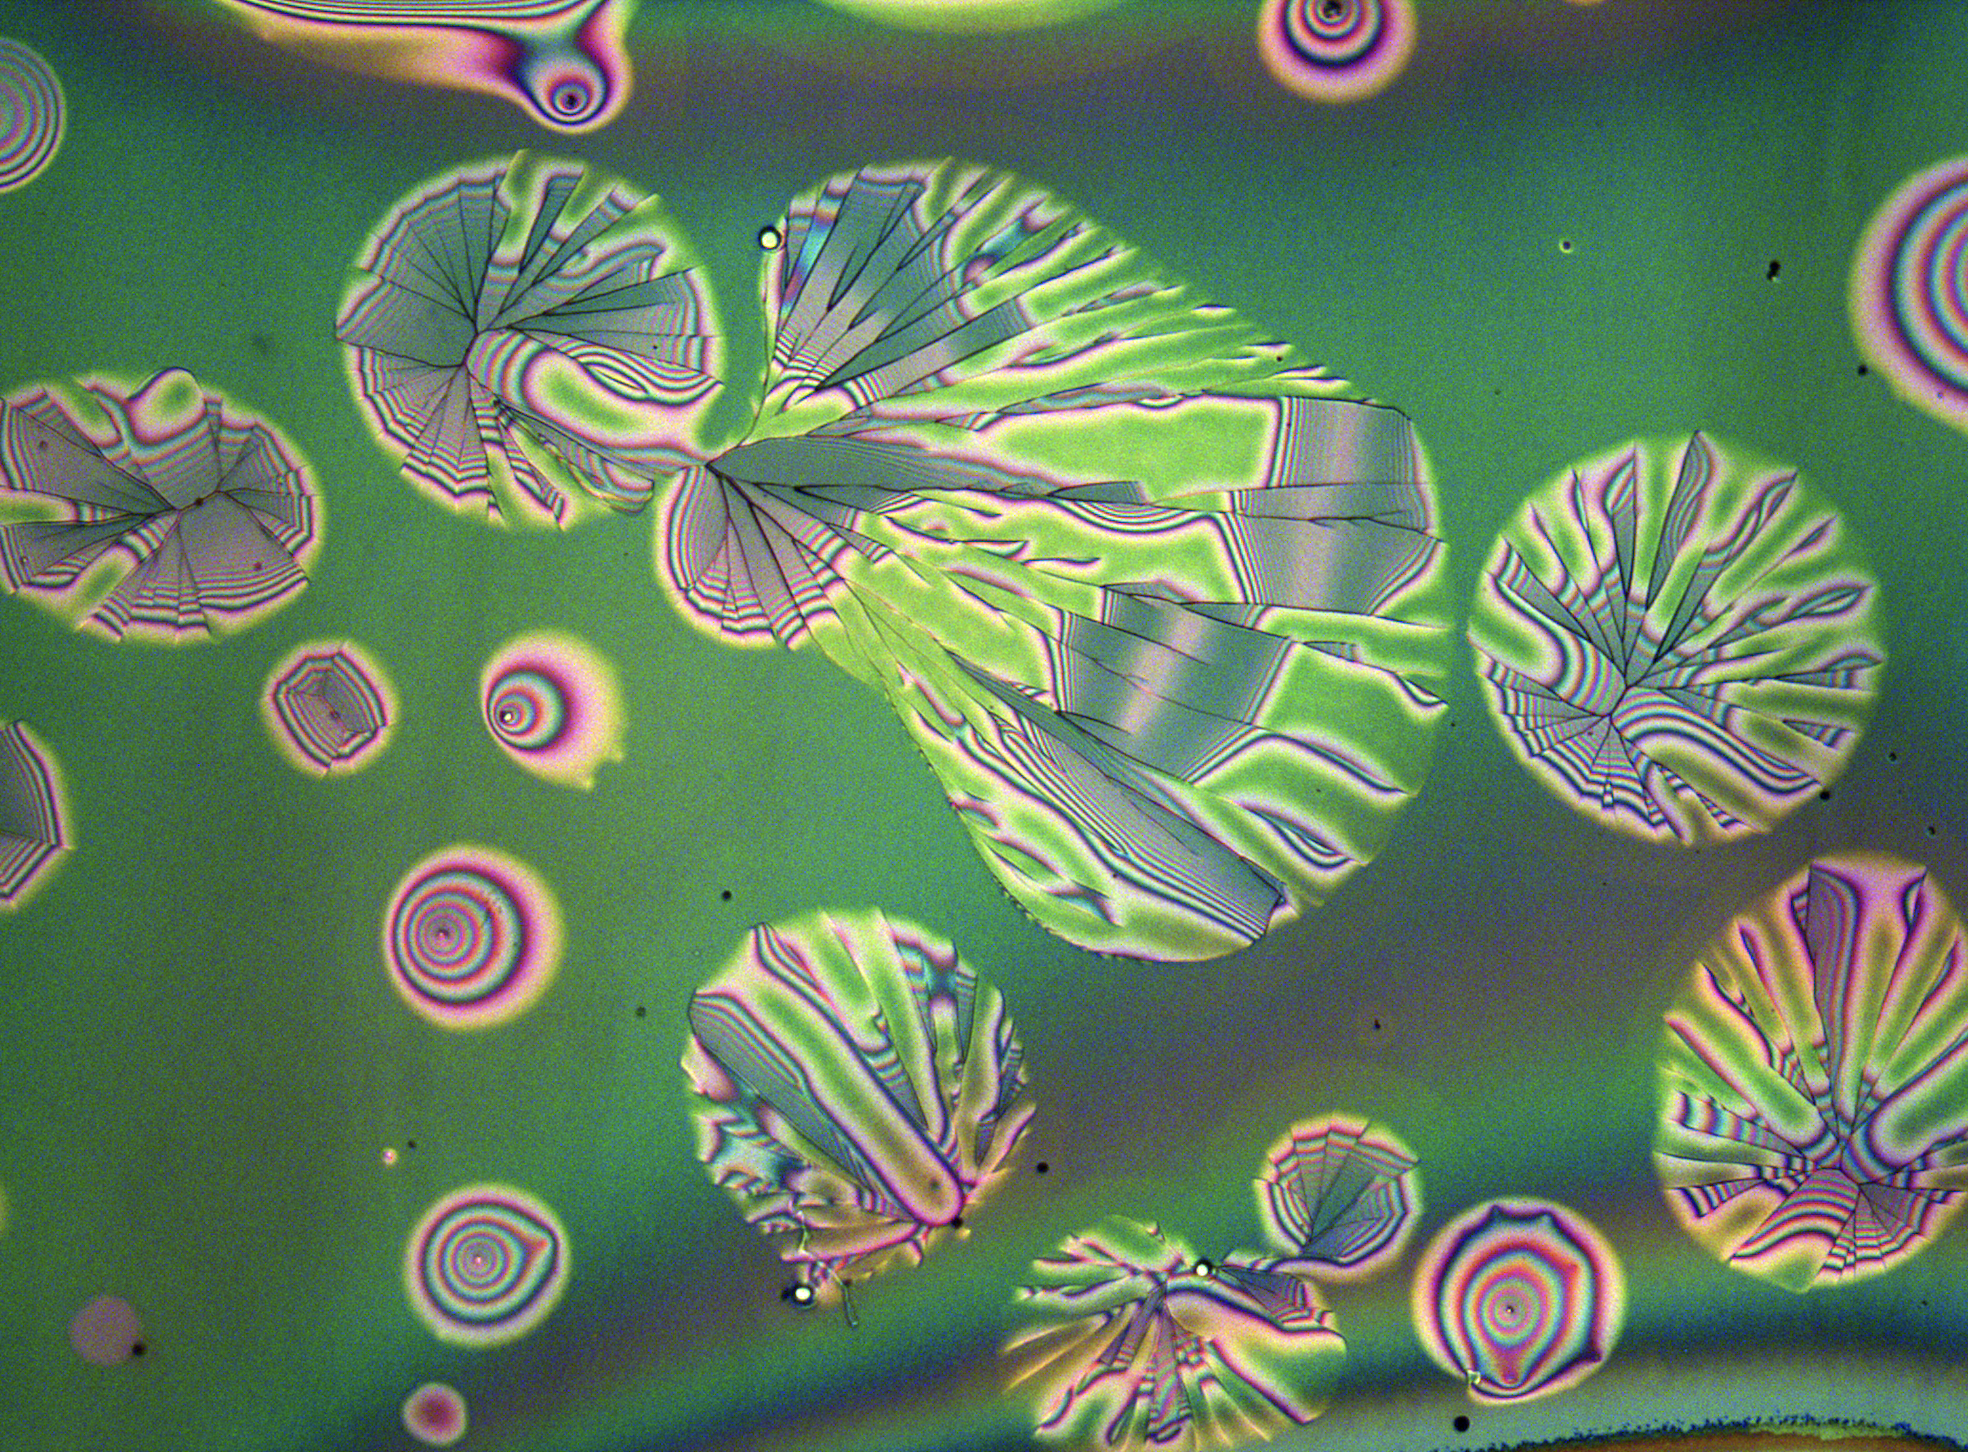
\includegraphics[width=0.45\textwidth]{figures/led_after_pecvd.png}
    \caption{Optical image of the LED.}
    \label{fig:led_optical}
\end{figure}



\subsection{Other Things}
We still need the following:
% list
\begin{itemize}
    \color{red}
    \item images of alingment marks
    \item IES test of LED. I-V curve
\end{itemize}


Results we will list:

\begin{enumerate}
    \color{olive}
    \item undercut in SEM image (done)
    \item etch depth for GaAs etch, 100 nm (done)
    \color{violet}
    \item alignment accuracy
    \item etch depth for AlGaAs etch, 3 um
    \item PECVD Si3N4 thickness vs. deposition time, reflection curve vs. wavelength (or at least the reflection minima for the final thickness and the reflectivity at 675 nm).
    \item Optical images of the sample after finishing steps in the PECVD independent work.
    \item Optical image of final LED
\end{enumerate}




% profilometer on GaAs etch
The wet etch of the dummy was done for XX seconds and gave a depth of 50 nm, thus the etching of the LED was done for twice as long at XX seconds and gave a depth of 100 nm.
This is an etch rate of \textbf{XXXXXXX} nm/s.
Two of the measured profilometer finger heights are shown in \autoref{fig:profilometer_GaAs_100nm_etch}.
The other measurements of the fingers gave similar results.
Before the etch the Au fingers was measured to be 250 nm high.
In the figure it is possible to see the etch edge, which is marked with the green line at 100 nm. 
The second green line is at 350 nm, which is the height of the finger after the etch.
A profilometer artifact is shown in \autoref{fig:Dummy_GaAs_80nm_etch_lost_contact}.



% figure LED_GaAs_100nm_etch.png
\begin{figure}[ht]
    \centering
    \includegraphics[width=0.45\textwidth]{figures/LED_GaAs_100nm_etch.png}
    \caption{
        Profilometer data plot of the GaAs top layer etch. 
        The etch was 100 nm deep, which is sufficient to get through the light absorbing layer.
        The plot shows an artifact on top of the finger to the left, but these were not examined further.
    }
    \label{fig:profilometer_GaAs_100nm_etch}
\end{figure}

% figure Dummy_GaAs_80nm_etch_lost_contact.png
\begin{figure}[ht]
    \centering
    \includegraphics[width=0.45\textwidth]{figures/Dummy_GaAs_80nm_etch_lost_contact.png}
    \caption{
        Profilometer data plot of GaAs dummy on the etch edge. 
        The etch depth here was 80 nm, which was deeper that around the fingers. 
        However, this plot shows an artifact in the profilometer, which is the curve starting at around 550 \textmu m.
        The upwards curve continues upwards outside the plot till 350 nm, which is higher than the finger height.
    }
    \label{fig:Dummy_GaAs_80nm_etch_lost_contact}
\end{figure}


% profilometer on AlGaAs etch

The deep AlGaAs wet etch for the mesas was done for 1 minute and 45 seconds and gave a depth of 3.1 um. 
The dummy was etched for 1 minute and 30 seconds and gave a depth of 2.9 um, and thus the LED was etched for 15 more seconds. 
The profilometer data was not extracted to be plotted. 
However, the etch rate was measured to be 30 nm/s.
\textbf{TODO: Should we plot the data??}

% still in nanolab???